\section{Analysis of the results}
In this section we are going to discuss the results of the top-k algorithm applied to the IMDb graphs. We are particularly interested in two factors:
\begin{itemize}
    \item The time needed to for the execution in function of different filtering values.
    \item The discrepancy on the results while varying the filtering values
\end{itemize}
The first one will tell us how much more efficient the algorithm is in terms of time, independently from the results. The second one is the metric to understand how accurate the filtered algorithm is. It's clear that even if we can compute the algorithm 100 times faster, it's of no use if the results are completely different from the real ones.\s

\nd The platform for the tests is \emph{a laptop}, so can not be considered precise due factors as thermal throttling. The CPU is an Intel(R) Core™ i7-8750H (6 cores, 12 threads), equipped with 16GB of DDR4 @2666 MHz RAM.

\subsection{Actors graph} \label{actors-graph}
Let's take into analysis the graph were each actors is a node and two nodes are linked the if they played in a movie together. In the case, during the filtering, we created the variable \texttt{MIN\textunderscore ACTORS}. This variable is the minimun number of movies that an actor/actress has to have done to be considered in the computation.

Varying this variable obviously affects the algorithm, in different way. The higher this variable is, the less actors we are taking into consideration. So, with a smaller graph, we are expecting better results in terms of time execution. On the other hand, we also can expect to have less accurate results. What we are going to discuss is how much changing \texttt{MIN\textunderscore ACTORS} affects this two factors

\subsubsection{Time of execution}

TO DO

\subsubsection{Discrepancy of the results}
We want to analyze how truthful our results are while varying \texttt{MIN\textunderscore ACTORS}. The methodology is simple: for each results (lists) we take the intersection of the two. This will return the number of elements in common. Knowing the length of the lists, we can find the number of elements not in common. \s

\nd A way to see this results is with a square matrix $n \times n, ~ A = (a_{ij})$, where $n$ is the number of different values that we gave to \texttt{MIN\textunderscore ACTORS} during the testing. In this way the $(i,j)$ position is the percentage of discrepancy between the results with \texttt{MIN\textunderscore ACTORS} set as $i$ and $j$ \s

\nd This analysis is implemented in python using the \texttt{pandas} and \texttt{numpy} libraries.

\lstinputlisting[language=c++]{code/closeness_analysis.py}

\nd Visualizing this analysis we obtain this

\begin{figure}[h] \label{matrix-a}
    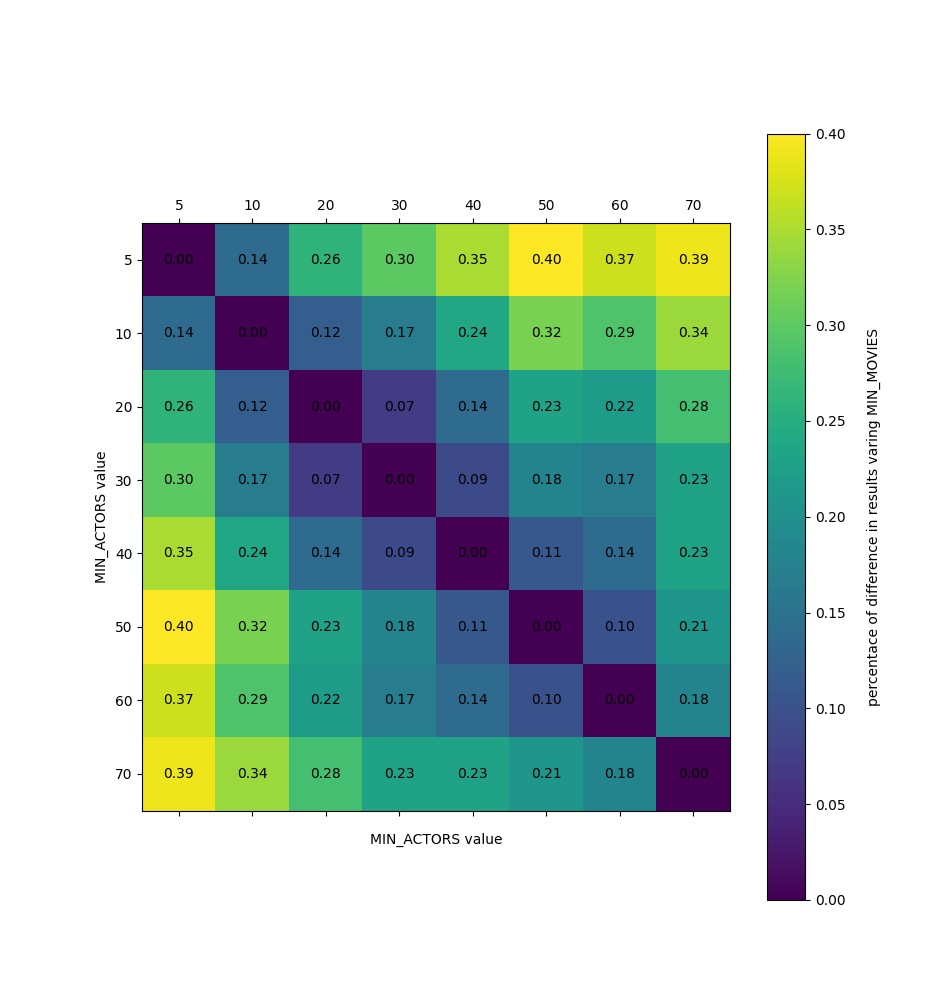
\includegraphics[width=12cm]{Figure_1.png}
    \caption{Discrepancy of the results on the actors graph in function of the minimum number of movies required to be considered as a node}
\end{figure}

\nd As expected, the matrix is symmetrical and the elements on the diagonal are all equal to zero. We can see clearly that with a lower value of \texttt{MIN\textunderscore ACTORS} the results are more precise. The discrepancy with \texttt{MIN\textunderscore ACTORS=10} is 14\% while being 39\% when \texttt{MIN\textunderscore ACTORS=70}. \s

\nd This is what we obtain confronting the top-k results when $k=100$. It's interesting to se how much the discrepancy change with different values of $k$. However, choosing a lower value for $k$ would not be useful for this type of analysis. Since we are looking at the not common elements of two lists, with a small length, we would get results biased by statistical straggling. \s

\textsc{Da fare: test con con k=500 e k=1000}

\s
\newpage
\subsection{Movies Graphs}
In this section we are taking into consideration the graph build over the movies and their common actors/actresses. Due to an elevated number of nodes, to optimize the performance during the execution in the section \ref{filtering} we introduced the variable \texttt{VOTES}. It represents the minimum number of votes (indifferently is positive or negative) that a movie need to have on the IMDb database to be considered as a node in our graph.

As seen during the analysis of the actors graph in \ref{actors-graph}, varying this kind of variables affects the results in many ways. All the observations made before are still valid for this case, I won't repeat them for shortness. As done before (\ref{matrix-a}), we are going to use a matrix to visualize and analyze the results
\s

% \lstinputlisting[language=c++]{code/closeness_analysis_2.py}

\nd Giving us:
\begin{figure}[H] \label{matrix-b}
    \centering
    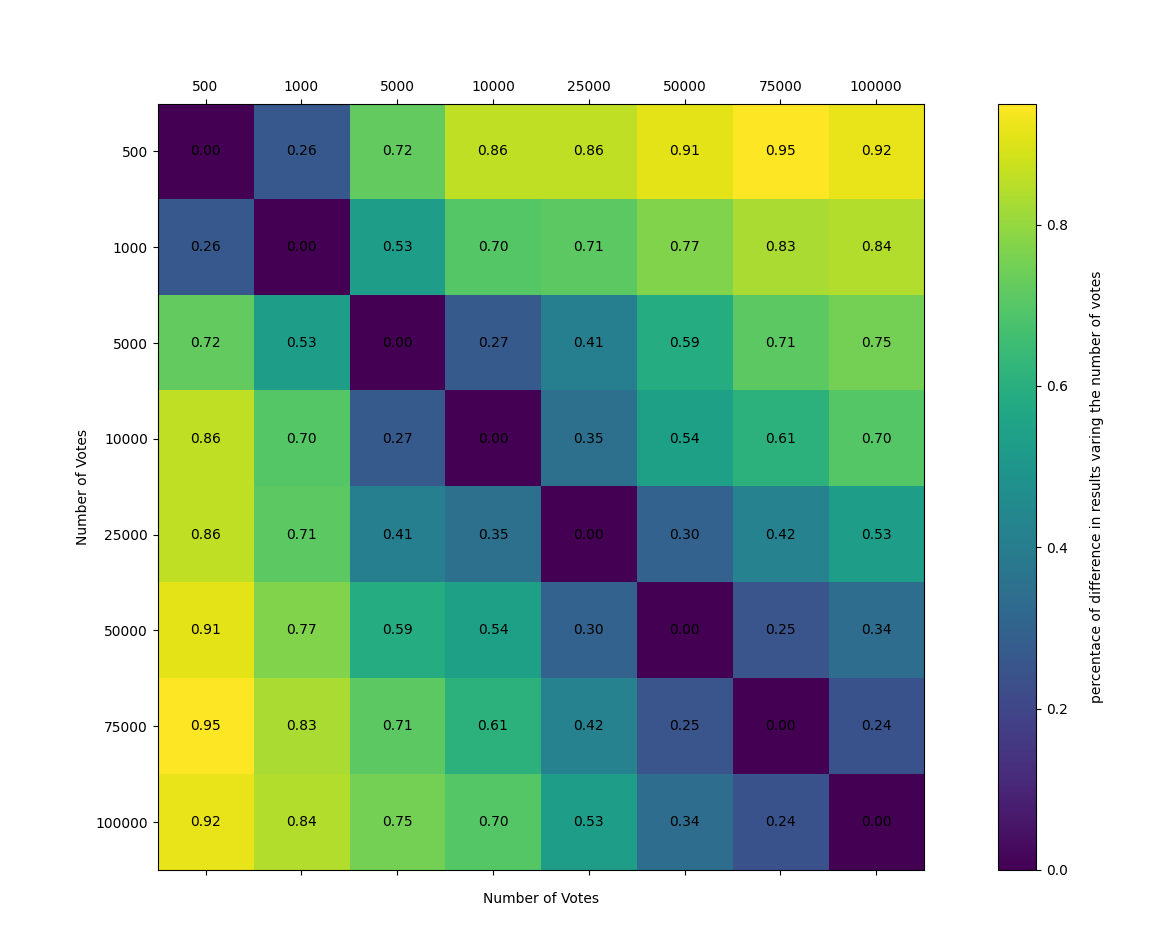
\includegraphics[width=13cm]{Figure_2.png}
    \caption{Discrepancy of the results on the movie graph in function of the minimum number of votes required to be considered as a node}
\end{figure}
\newpage
\lstinputlisting[language=c++]{code/closeness_analysis_2.py}

\s \nd \emph{Dire qualcosa sull'analisi, ma andrebbe rifatta perché i valori non vanno bene}
